\documentclass[12pt,a4paper]{article}
\usepackage{cmap} % Makes the PDF copiable. See http://tex.stackexchange.com/a/64198/25761
\usepackage[T1]{fontenc}
\usepackage[brazil]{babel}
\usepackage[utf8]{inputenc}
\usepackage{amsmath}
\usepackage{amsfonts}
\usepackage{amssymb}
\usepackage{amsthm}
\usepackage{textcomp} % \degree
\usepackage{gensymb} % \degree
\usepackage[usenames,svgnames,dvipsnames]{xcolor}
\usepackage{hyperref}
\usepackage{multicol}
\usepackage{graphicx}
\usepackage[margin=2cm]{geometry}
\usepackage{systeme}

\hypersetup{
    colorlinks = true,
    allcolors = {blue}
}

% TODO: Consider using exsheets
% http://linorg.usp.br/CTAN/macros/latex/contrib/exsheets/exsheets_en.pdf
%
% http://ctan.org/tex-archive/macros/latex/contrib/exercise/
% Options: answerdelayed,lastexercise,noanswer
\usepackage[answerdelayed,lastexercise]{exercise}

\addto\captionsbrazil{%
\def\listexercisename{Lista de exerc\'icios}%
\def\ExerciseName{Exerc\'icio}%
\def\AnswerName{Solu\c{c}\~ao do exerc\'icio}%
\def\ExerciseListName{Ex.}%
\def\AnswerListName{Solu\c{c}\~ao}%
\def\ExePartName{Parte}%
\def\ArticleOf{de\ }%
}

\renewcommand{\ExerciseHeaderTitle}{(\ExerciseTitle)\ }
\renewcommand{\ExerciseListHeader}{%\ExerciseHeaderDifficulty%
\textbf{%\ExerciseListName\
\ExerciseHeaderNB.\ %
%\ --- \ 
\ExerciseHeaderTitle}%
%\ExerciseHeaderOrigin
\ignorespaces}
\renewcommand{\AnswerListHeader}{\textbf{\ExerciseHeaderNB.\ (\AnswerListName)\ }}

\renewcommand{\theenumi}{\alph{enumi}}
\renewcommand\labelenumi{(\theenumi) }

\newcommand*\tipo{Prova II}
\newcommand*\turma{PRO112-04U}
\newcommand*\disciplina{CAN0001}
\newcommand*\eu{Helder G. G. de Lima}
\newcommand*\data{16/05/2017}

\author{\eu}
\title{\tipo - \disciplina}
\date{\data}

\begin{document}
\thispagestyle{empty}
\newgeometry{margin=2cm,bottom=0.5cm}
\begin{center}

\includegraphics[width=9.0cm]{marca} \\
\textbf{\tipo\ (\disciplina / \turma)} \\
Prof. \eu\footnote{
Este é um material de acesso livre distribuído sob os termos da licença \href{https://creativecommons.org/licenses/by-sa/4.0/deed.pt_BR}{Creative Commons Atribuição-CompartilhaIgual 4.0 Internacional}}
\end{center}

\noindent Nome do(a) aluno(a): \underline{\hspace{9,7cm}} Data: \underline{\data}

%\section*{Instruções}
\begin{center}\fbox{
\begin{minipage}{14cm}

{\footnotesize
\begin{itemize}
\renewcommand{\theenumi}{\Roman{enumi}}
\item Identifique-se em todas as folhas.
\item Mantenha o celular e os demais equipamentos eletrônicos desligados durante a prova.
\item Justifique cada resposta com cálculos ou argumentos baseados na teoria estudada.
\item Ao escrever números decimais, arredonde-os com 4 casas depois da vírgula.
\item Resolva apenas os itens de que precisar para somar 10,0 pontos.
\end{itemize}
}

\end{minipage}
}
\end{center}

%\section*{Questões}
\begin{ExerciseList}
\Exercise[title={2,5}]
Utilize a fatoração $A = LU$ para resolver o sistema
$
\systeme{
 4x_1 + 3x_2 + 2x_3 + 2x_4 = 0,  
 4x_1 + 5x_2 + 5x_3 + 6x_4 = 3,
-4x_1 - 3x_2 - 3x_3        = 0,
        4x_2 + 6x_3 + 6x_4 = 5.
}
$
\Answer Pode-se escrever $A = LU$, sendo
$
L = 
\begin{bmatrix}
 1 & 0 & 0 & 0 \\
 1 & 1 & 0 & 0 \\
-1 & 0 & 1 & 0 \\
 0 & 2 & 0 & 1
\end{bmatrix}
$
e
$
U = 
\begin{bmatrix}
4 & 3 &  2 &  2 \\
0 & 2 &  3 &  4 \\
0 & 0 & -1 &  2 \\
0 & 0 &  0 & -2
\end{bmatrix}
$.
Para obter $X$ tal que $AX = B$, calcula-se $Y$ tal que $LY = B$ e $X$ tal que $UX = Y$. Assim,
\[
\systeme{
 y_1                      = 0,  
 y_1 +  y_2               = 3,
-y_1         + y_3        = 0,
       2y_2        + 6y_4 = 5
}
\Leftrightarrow
Y =
\begin{bmatrix}
 0 \\
 3 \\
 0 \\
-1
\end{bmatrix}
\text{ e }
\systeme{
4x_1 + 3x_2 + 2x_3 + 2x_4 = 0,
       2x_2 + 3x_3 + 4x_4 = 3,
            -  x_3 + 2x_4 = 0,
                   - 2x_4 = -1
}
\Leftrightarrow
X = 
\begin{bmatrix}
 0 \\
-1 \\
 1 \\
1/2
\end{bmatrix}
\]



\Exercise[title={2,5}]
Obtenha, usando 3 iterações do método de Jacobi, uma solução aproximada do sistema
\[
\systeme{
4x_1 - 2x_3        =-4,
 x_1 + 3x_2        = 4,
-x_1 +  x_2 + 3x_3 = 5.
}
\]
Use a aproximação inicial $x_1^{(0)} = x_2^{(0)} = x_3^{(0)} = 0$, e estime o erro relativo percentual da solução.
\Answer Ao aplicar o método de Jacobi, são utilizadas as seguintes equações:
\[
\begin{cases}
x_1^{(k)} = (-4 + 2x_3^{(k-1)})/4\\
x_2^{(k)} = (4 - x_1^{(k-1)})/3\\
x_3^{(k)} = (5 + x_1^{(k-1)} - x_2^{(k-1)})/3.
\end{cases}
\]
Os valores obtidos a cada iteração são os seguintes:
\begin{center}
\begin{tabular}{|r|r|r|r|r|}
\hline
$\mathbf{k}$     & 1 & 2 & 3 \\
\hline
$\mathbf{x_1^{(k)}}$ &-1.0000 &-0.1667 & -0.5555 \\
\hline
$\mathbf{x_2^{(k)}}$ & 1.3333 & 1.6667 &  1.3889 \\
\hline
$\mathbf{x_3^{(k)}}$ & 1.6667 & 0.8889 &  1.0555 \\
\hline
\end{tabular}
\end{center}
\medskip
Na terceira iteração, o erro absoluto é estimado como
\begin{align*}
\varepsilon_{abs}
& \approx || x^{(3)} - x^{(2)} ||
= \max\{|-0.5555 -(-0.1667)|,
        | 1.3889 -  1.6667|,
        | 1.0555 -  0.8889|\}\\
& = \max\{ |-0.3889|, |-0.2778|, |0.1666| \}
= 0.3889.
\end{align*}
Então o erro relativo percentual é:
\[
\varepsilon_{per}
\approx
\frac{ || x^{(3)} - x^{(2)} || }{ || x^{(3)} || } \times 100 \%
= \frac{ 0.3889 }{ 1.3889 } \times 100 \% 
= 0.2800 \times 100 \%
= 28.00 \%.
\]

\Exercise[title={2,5}]
Verifique se é garantido que o método de Gauss-Seidel convergirá, se for aplicado a
\[
\systeme{
 4x_1 + 3x_2 = 5,
-2x_1 + 5x_2 = 4.
}
\]
Em caso afirmativo, determine se com 3 iterações do método, partindo de $x_1^{(0)} = x_2^{(0)} = 0$, é possível obter um erro relativo percentual $\varepsilon < 50\%$.
\Answer Para que o método de Gauss-Seidel convirja é suficiente que a matriz de coeficientes do sistema seja estritamente diagonal dominante. Sendo
$
A =
\begin{bmatrix}
4 & 3 \\ -2 & 5
\end{bmatrix}
$, tem-se:
\begin{align*}
|a_{11}| & = 4 > 3 = |3| = \sum_{j \neq 1} |a_{1j}|,\\
|a_{22}| & = 5 > 2 = |-2| = \sum_{j \neq 2} |a_{2j}|.
\end{align*}
Logo, $A$ é estritamente diagonal dominante e o método converge. Para aplicá-lo, são utilizadas as seguintes equações:
\[
\begin{cases}
x_1^{(k)} = (5 -3x_2^{(k-1)})/4\\
x_2^{(k)} = (4 +2x_1^{(k)})/5.
\end{cases}
\]
Os valores obtidos a cada iteração são os seguintes:
\begin{center}
\begin{tabular}{|r|r|r|r|r|}
\hline
$\mathbf{k}$     & 1 & 2 & 3 \\
\hline
$\mathbf{x_1^{(k)}}$ & 1.2500 & 0.2750 & 0.5675 \\
\hline
$\mathbf{x_2^{(k)}}$ & 1.3000 & 0.9100 & 1.0270 \\
\hline
\end{tabular}
\end{center}
\medskip
Na terceira iteração, a estimativa para o erro absoluto é
\begin{align*}
\varepsilon_{abs}
& \approx || x^{(3)} - x^{(2)} ||
= \max\{| 0.5675 - 0.2750 |,
        | 1.0270 - 0.9100|\}\\
& = \max\{ |0.2925|, |0.1170|\}
= 0.2925.
\end{align*}
Então o erro relativo percentual é:
\[
\varepsilon_{per}
\approx
\frac{ || x^{(3)} - x^{(2)} || }{ || x^{(3)} || } \times 100 \%
= \frac{ 0.2925 }{ 1.0270 } \times 100 \% 
= 0.2848 \times 100 \%
= 28.48 \%.
\]


\Exercise[title={2,5}]
Os números $T_2 = 3$, $T_3 = 6$, $T_4 = 10$ e $T_5 = 15$ são chamados de \textit{números triangulares} pois é possível distribuir $T_n$ objetos em forma de um triângulo equilátero, com $n$ objetos em cada lado do triângulo. Por exemplo, para $n \in \{2, 3, 4\}$, estes são os triângulos resultantes:
\begin{center}
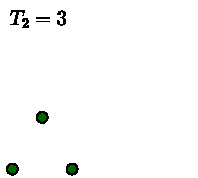
\includegraphics[width=2.3cm]{img/prova-2-pro-t2.pdf}
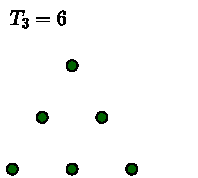
\includegraphics[width=2.3cm]{img/prova-2-pro-t3.pdf}
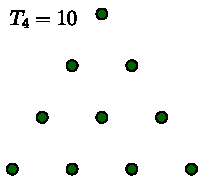
\includegraphics[width=2.3cm]{img/prova-2-pro-t4.pdf}
\end{center}

Utilize os polinômios interpoladores de Lagrange para obter um polinômio $p$ tal que $p(n) = T_n$, para $n \in \{2,3,4\}$. Qual é o erro absoluto cometido ao usar este polinômio para estimar $T_5$?
\Answer O polinômio interpolador é dado por
\begin{align*}
p(x)
& = 3 L_1(x)+ 6L_2(x)+ 10L_3(x) \\
& = 3 \frac{(x-3)(x-4)}{(2-3)(2-4)}
  + 6 \frac{(x-2)(x-4)}{(3-2)(3-4)}
 + 10 \frac{(x-2)(x-3)}{(4-2)(4-3)} \\
& = \frac{3}{2}(x^2 - 7 x + 12)
  - 6 (x^2 - 6 x + 8)
  + \frac{10}{2} (x^2 - 5x + 6)\\
& = \frac{x^2}{2} + \frac{x}{2}.
\end{align*}
Usando este polinômio, obtém-se $p(5) = \frac{25}{2} + \frac{5}{2} = 15 = T_5$, então o erro absoluto é zero.

\Exercise[title={2,5}]
Se forem utilizados os pontos $x_0=-1$, $x_1=0$, $x_2=1$ e $x_3=8$ para encontrar, por diferenças divididas, um polinômio $p(x)$ que interpola a função $f(x) = \sqrt[3]{x}$, qual dos seguintes valores poderá ser estimado com o menor erro relativo: $f(2) = \sqrt[3]{2}$ ou $f(7) = \sqrt[3]{7}$?
\Answer Usando os pontos dados obtém-se:
\[
	\begin{array}{cccccc}
   x_i & y_i=f[x_i] & f[x_i,x_{i+1}] & f[x_i,x_{i+1},x_{i+2}]  & f[x_i,x_{i+1},x_{i+2},x_{i+3}] \\
   -1 & \mathbf{-1} \\
	    &     & \mathbf{1} \\
	0 & 0 &             & \mathbf{0}\\
	    &     & 1 &              & \mathbf{\frac{-1}{84}=-0.0119}. \\
	1 & 1 &             & \frac{-3}{28}=-0.1071\\
	    &     & \frac{1}{7}=0.1429\\
	8 & 2
	\end{array}
\]
Então:
\begin{align*}
p(x)
= -1 + 1(x-(-1)) + 0 (x-(-1))(x-0) + \frac{-1}{84}(x-(-1))(x-0)(x-1)
= \frac{85}{84}x - \frac{x^3}{84}.
\end{align*}
Usando este polinômio para estimar os valores pedidos, resulta que:
\begin{itemize}
\item $p(2) = \frac{170}{84} - \frac{8}{84} = \frac{27}{14} \approx 1.9286$, e neste caso $\varepsilon_{rel}
= \frac{ |\sqrt[3]{2} - \frac{27}{14}| }{ |\sqrt[3]{2}| }
\approx \frac{ |1.2599 - 1.9286| }{ |1.2599| } = 0.5308$
\item $p(7) = \frac{170}{84} - \frac{8}{84} = 3$, e neste caso $\varepsilon_{rel}
= \frac{ |\sqrt[3]{7} - 3| }{ |\sqrt[3]{7}| }
\approx \frac{ |1.9129 - 3| }{ |1.9129| } = 0.5683$
\end{itemize}
Assim, o erro é menor ao estimar $\sqrt[3]{2}$.
\end{ExerciseList}

\vspace{0.4cm}
\begin{center}
BOA PROVA!
\end{center}

\newpage
\restoregeometry
\section*{Respostas}
\shipoutAnswer
\end{document}
